% Motor: XeLaTeX. Sesión 23 - material docente UTP.
% Estructura docente de la Sesión 22.
\documentclass[aspectratio=169,10pt,c]{beamer}
% Reutiliza sin cambios la identidad visual UTP validada en la Sesion 08.
% Reutiliza sin cambios la identidad visual UTP validada en la Sesion 05.
% La segunda ruta permite compartir los assets comunes sin duplicar binarios.
% !TEX root = slides.tex
% Preambulo comun: estilo UTP, colores, fuentes, plantillas de beamer y
% comandos de apoyo didactico. Se carga desde slides.tex tras \documentclass.

% La opción "c" de beamer reparte el espacio libre 1:1.5 (arriba:abajo), por lo
% que el contenido queda por encima del centro. Igualamos ambos rellenos.
\makeatletter
\define@key{beamerframe}{c}[true]{%
  \beamer@frametopskip=0pt plus 1fill\relax%
  \beamer@framebottomskip=0pt plus 1fill\relax%
  \beamer@frametopskipautobreak=0pt plus .5\paperheight\relax%
  \beamer@framebottomskipautobreak=0pt plus .5\paperheight\relax%
}
\makeatother

\usepackage{graphicx}
\usepackage{tikz}
\usepackage{xcolor}
\usepackage{iftex}

\ifPDFTeX
  \usepackage[utf8]{inputenc}
  \usepackage[T1]{fontenc}
  \usepackage{lmodern}          % tipografia escalable para el respaldo con pdflatex
  \renewcommand{\familydefault}{\sfdefault}
\else
  \usepackage{fontspec}
  \IfFontExistsTF{Arial}
    {\setsansfont{Arial}[BoldFont={Arial Bold}]}
    {\setsansfont{Helvetica}[BoldFont={Helvetica Bold}]}
\fi

\usepackage[spanish,es-nodecimaldot]{babel}
\usepackage{microtype}
\usepackage{booktabs}
\usepackage{array}
\usetikzlibrary{arrows.meta,positioning,fit,calc,shapes.geometric}

\graphicspath{{assets/}}

% ---------- Identidad visual UTP ----------
\definecolor{utpRojo}{HTML}{C42B35}
\definecolor{utpNegro}{HTML}{111111}
\definecolor{utpGris}{HTML}{5F5F5F}
\definecolor{utpGrisMedio}{HTML}{9A9A9A}
\definecolor{utpGrisClaro}{HTML}{F1F1F1}

\usetheme{default}
\setbeamercolor{normal text}{fg=utpNegro,bg=white}
\setbeamercolor{structure}{fg=utpRojo}
\setbeamercolor{frametitle}{fg=utpNegro,bg=white}
\setbeamercolor{title}{fg=utpNegro}
\setbeamercolor{subtitle}{fg=utpNegro}
\setbeamercolor{author}{fg=utpNegro}
\setbeamercolor{date}{fg=utpNegro}
\setbeamercolor{block title}{fg=white,bg=utpNegro}
\setbeamercolor{block body}{fg=utpNegro,bg=utpGrisClaro}
\setbeamercolor{alertblock title}{fg=white,bg=utpRojo}
\setbeamercolor{alertblock body}{fg=utpNegro,bg=utpRojo!7}
\setbeamercolor{exampleblock title}{fg=white,bg=utpGris}
\setbeamercolor{exampleblock body}{fg=utpNegro,bg=utpGris!8}
\setbeamercolor{terminal}{fg=white,bg=utpNegro}

\setbeamerfont{title}{series=\bfseries,size=\fontsize{19.5}{22.5}\selectfont}
\setbeamerfont{subtitle}{size=\fontsize{11.5}{13.5}\selectfont}
\setbeamerfont{date}{series=\bfseries,size=\fontsize{11.5}{13.5}\selectfont}
\setbeamerfont{author}{size=\fontsize{10.5}{12.5}\selectfont}
\setbeamerfont{frametitle}{series=\bfseries,size=\large}
\setbeamerfont{block title}{series=\bfseries,size=\small}
\setbeamerfont{block body}{size=\normalsize}

\setbeamertemplate{navigation symbols}{}
\setbeamertemplate{headline}{}
\setbeamertemplate{blocks}[default]
\setbeamertemplate{itemize item}{\color{utpRojo}\small\raise.15ex\hbox{$\blacktriangleright$}}
\setbeamertemplate{itemize subitem}{\color{utpGris}\scriptsize$\bullet$}
\setbeamertemplate{enumerate item}{\color{utpRojo}\insertenumlabel.}
\setbeamertemplate{background canvas}{\color{white}\rule{\paperwidth}{\paperheight}}

% Título de diapositiva: negrita negra a la izquierda, logo UTP a la derecha
\setbeamertemplate{frametitle}{%
  \begin{tikzpicture}[remember picture,overlay]
    \node[anchor=north east,inner sep=0pt]
      at ([xshift=-7mm,yshift=-5.5mm]current page.north east)
      {\includegraphics[width=17mm]{utp-logo.png}};
  \end{tikzpicture}%
  \vspace{1.2mm}%
  \begin{minipage}[t]{.80\textwidth}\raggedright\insertframetitle\end{minipage}\par
  \vspace{1.1mm}{\color{utpRojo}\rule{\textwidth}{1.1pt}}
}

% Solo numeración discreta; la plantilla UTP no lleva pie de página
\setbeamertemplate{footline}{%
  \hfill{\color{utpGrisMedio}\scriptsize\insertframenumber}\hspace{6mm}\vspace{2.5mm}%
}

% Portada UTP
\setbeamertemplate{title page}{%
  \begin{tikzpicture}[remember picture,overlay]
    \node[anchor=center,inner sep=0pt] at (current page.center) {%
      \includegraphics[width=\paperwidth,height=\paperheight]{utp-cover-bg.jpeg}%
    };
    \node[anchor=north,align=center,text=utpNegro,inner sep=0pt,
      text width=145mm,font=\usebeamerfont{title}]
      at ([yshift=-25.2mm]current page.north) {\inserttitle};
    \node[anchor=north,align=center,text=utpNegro,inner sep=0pt,
      text width=142mm,font=\usebeamerfont{subtitle}]
      at ([yshift=-38.2mm]current page.north) {\insertsubtitle};
    \node[anchor=north,align=center,text=utpNegro,inner sep=0pt,
      font=\usebeamerfont{date}]
      at ([yshift=-50.4mm]current page.north) {\insertdate};
    \node[anchor=north,align=center,text=utpNegro,inner sep=0pt,
      font=\usebeamerfont{author}]
      at ([yshift=-58.4mm]current page.north) {\insertauthor};
  \end{tikzpicture}%
}

% ---------- Comandos de apoyo didáctico ----------
\newcommand{\concepto}[2]{%
  \begin{block}{#1}\large #2\end{block}}
\newcommand{\pregunta}[1]{%
  \begin{alertblock}{Decide y explica}#1\end{alertblock}}
\newcommand{\analogia}[1]{%
  \begin{exampleblock}{En palabras simples}\small #1\end{exampleblock}}
\newcommand{\enlarealidad}[1]{%
  \begin{block}{Cómo se ve en la realidad}\small #1\end{block}}
\newcommand{\ojo}[1]{%
  \begin{alertblock}{Ojo con esto}\small #1\end{alertblock}}
\newcommand{\apoyo}{{\normalfont\footnotesize\color{utpGris}~· material de apoyo}}
\newcommand{\marca}[1]{\tikz[baseline=(m.base)]{%
  \node[rounded corners=1.5pt,fill=utpGrisClaro,draw=utpGrisMedio,inner xsep=3pt,inner ysep=1.5pt,
        font=\footnotesize] (m) {#1};}}
\newenvironment{terminal}{%
  \begin{beamercolorbox}[wd=\linewidth,sep=5pt,rounded=true]{terminal}%
  \ttfamily\small\ignorespaces}{%
  \end{beamercolorbox}}

\tikzset{
  caja/.style={draw=utpNegro, very thick, rounded corners=1.5pt, fill=white,
    align=center, minimum height=0.72cm, inner sep=5pt, font=\small},
  cajaazul/.style={caja, draw=utpGris, fill=white},
  cajaverde/.style={caja, draw=utpNegro, fill=utpGrisClaro},
  cajanaranja/.style={caja, draw=utpRojo!75, fill=utpRojo!7},
  flecha/.style={-{Stealth[length=2.3mm]}, very thick, draw=utpNegro},
  flechavuelta/.style={{Stealth[length=2.3mm]}-{Stealth[length=2.3mm]}, very thick, draw=utpNegro}
}

\graphicspath{{../../Sesion05/slides/assets/}}



\graphicspath{{assets/}{../../Sesion05/slides/assets/}}

\title{Integración de Servicios Cloud GCP}
\subtitle{Bases de datos en Google Cloud: tipos, usos y Cloud SQL}
\date{Semana 12 - Sesión 23}
\author{Rel Guzman}

\newcommand{\separador}[2]{%
\begin{frame}[plain]
\vfill
\begin{center}
{\fontsize{29}{34}\selectfont\bfseries #1}\par
\vspace{2mm}
{\small #2}\par
\vspace{4mm}
{\color{utpRojo}\rule{8.5cm}{1.2pt}}
\end{center}
\vfill
\end{frame}}

\begin{document}

{\setbeamertemplate{footline}{}\maketitle}

% 2
\begin{frame}{Revisión: IAM en una frase}
\begin{center}
\begin{tikzpicture}[font=\small,
 caja/.style={draw=utpRojo,rounded corners=4pt,minimum width=3.0cm,minimum height=1.1cm,align=center}]
  \node[caja,fill=utpRojo!25] (q) at (0,0) {\textbf{Laura}\\\footnotesize quién};
  \node[caja,fill=white,very thick] (r) at (4.6,0) {\textbf{Storage Object Viewer}\\\footnotesize qué puede hacer};
  \node[caja,fill=utpRojo!10] (s) at (9.2,0) {\textbf{Bucket de facturas}\\\footnotesize sobre qué};
  \draw[-latex,thick] (q) -- (r);
  \draw[-latex,thick] (r) -- (s);
\end{tikzpicture}
\end{center}
\begin{block}{Se lee así}
\small ``Laura puede ver y descargar los PDF del bucket de facturas''.
\end{block}
\begin{alertblock}{Pregunta rápida}
\small Laura emite facturas desde la aplicación, pero en el bucket solo puede ver y descargar. Entonces, ¿quién guarda el PDF en el bucket y con qué identidad?
\end{alertblock}
\end{frame}

% 3
\begin{frame}{Revisión: dos niveles de permisos}
\begin{center}
\begin{tikzpicture}[font=\small,
 caja/.style={draw=utpRojo,rounded corners=4pt,minimum width=2.6cm,minimum height=1.1cm,align=center}]
  \node[caja,fill=utpRojo!25] (l) at (0,0) {\textbf{Laura}\\\footnotesize navegador};
  \node[caja,fill=white,very thick] (v) at (5.4,0) {\textbf{Aplicación}\\\footnotesize VM con cuenta\\[-1pt]\footnotesize de servicio};
  \node[caja,fill=utpRojo!10] (b) at (10.8,0) {\textbf{Bucket}\\\footnotesize PDF de facturas};
  \draw[-latex,thick] (l) -- node[above,font=\footnotesize,align=center] {\textbf{1} emite\\la factura} (v);
  \draw[-latex,thick] (v) -- node[above,font=\footnotesize,align=center] {\textbf{2} guarda\\el PDF} node[below,font=\scriptsize,align=center] {rol de la cuenta\\de servicio:\\Storage Object Creator} (b);
  \draw[latex-,thick,dashed] (l.south) to[bend right=14] node[below,font=\footnotesize,align=center] {Laura descarga el PDF\\\scriptsize rol de Laura: Storage Object Viewer} (b.south);
\end{tikzpicture}
\end{center}
\begin{columns}[T,onlytextwidth]
\column{.48\textwidth}
\begin{block}{Nivel 1: la aplicación}
\small Sus reglas deciden qué hace Laura dentro de ella: \textbf{emitir} facturas.
\end{block}
\column{.48\textwidth}
\begin{block}{Nivel 2: IAM en Google Cloud}
\small Decide qué identidad toca cada recurso: la VM \textbf{crea} PDF; Laura solo los \textbf{ve y descarga}.
\end{block}
\end{columns}
\par\vspace{2mm}
\begin{alertblock}{¿Quién guarda el PDF en el bucket y con qué identidad?}
\small La \textbf{aplicación en la VM}, con su cuenta de servicio \texttt{sa-generador-facturas}, que tiene \texttt{Storage Object Creator}. Laura crea facturas a través de la aplicación, pero nunca escribe directo en el bucket.
\end{alertblock}
\end{frame}

% 4
\begin{frame}{Revisión: lo que el bucket no responde}
\begin{center}
\begin{tikzpicture}[font=\small,
 pdf/.style={draw=utpRojo,fill=white,minimum width=0.9cm,minimum height=1.1cm,font=\scriptsize}]
  \node[font=\small\bfseries] at (2.1,1.9) {El gerente pregunta};
  \node[draw=utpRojo,rounded corners=4pt,fill=utpRojo!10,align=center,minimum width=4.6cm,minimum height=0.9cm] at (2.1,1.1) {¿Cuánto le vendimos a Ana en marzo?};
  \foreach \i in {0,...,5} \node[pdf] at (0.1+\i*0.8,-0.4-0.08*\i) {PDF};
  \node[font=\footnotesize,align=center] at (2.1,-1.7) {Con solo el bucket: abrir\\cada PDF y sumar a mano};
  \draw[-latex,very thick,utpRojo] (5.6,0) -- (7.0,0);
  \node[draw=utpRojo,rounded corners=4pt,fill=white,very thick,align=left,font=\footnotesize] at (9.8,0.1)
   {\textbf{factura} \quad \textbf{cliente} \quad \textbf{monto}\\
    F-101 \qquad Ana \qquad\ \ 250\\
    F-102 \qquad Luis \qquad\ \ \ 80\\
    F-103 \qquad Ana \qquad\ \ 120};
  \node[font=\footnotesize,align=center] at (9.8,-1.7) {Con una base de datos:\\\textbf{370} al instante};
\end{tikzpicture}
\end{center}
\begin{alertblock}{La idea de hoy}
\small El bucket guarda \textbf{archivos}. Para buscar y sumar \textbf{datos} se usa una \textbf{base de datos}.
\end{alertblock}
\end{frame}

% 4
\begin{frame}[c]
\begin{block}{Logro de la sesión}
Al finalizar, podrás explicar qué es una \textbf{base de datos}, reconocer los \textbf{tipos} que ofrece Google Cloud y para qué sirve cada uno, y crear una base de datos en \textbf{Cloud SQL} a la que se conecta una aplicación.
\end{block}
\end{frame}

% 5
\begin{frame}{Saberes previos}
\begin{itemize}\setlength\itemsep{11pt}
  \item La agenda de contactos de tu celular: ¿qué datos guarda de cada persona? ¿Cómo encuentras a alguien entre 500 contactos?
  \item ¿Qué diferencia hay entre anotar pedidos en una hoja de cálculo y que una tienda en línea los registre sola?
\end{itemize}
\end{frame}

% 6
\begin{frame}[c]{Utilidad de esta sesión}
\begin{center}
\begin{minipage}{.84\textwidth}
{\large Casi toda aplicación guarda datos: usuarios, pedidos, pagos, citas. Si eliges bien \textbf{qué tipo de base de datos} usar y dejas que Google la \textbf{administre}, tu equipo se dedica a la aplicación y no a cuidar un servidor de base de datos.}
\end{minipage}
\end{center}
\end{frame}

% 7
\separador{Parte 1: tipos de bases de datos}{Qué guarda cada una y para qué sirve}

% 8
\begin{frame}{Dos grandes familias}
\begin{columns}[T,onlytextwidth]
\column{.48\textwidth}
\centering
{\large\bfseries Relacional}\par\vspace{1mm}
{\small Tablas, como una hoja de cálculo ordenada}\par\vspace{3mm}
\begin{tikzpicture}[font=\footnotesize]
  \fill[utpRojo!25] (0,1.5) rectangle (4.5,2.0);
  \draw[utpRojo,thick] (0,0) grid[xstep=1.5,ystep=0.5] (4.5,2.0);
  \node at (0.75,1.75) {\textbf{cliente}};
  \node at (2.25,1.75) {\textbf{monto}};
  \node at (3.75,1.75) {\textbf{fecha}};
  \node at (0.75,1.25) {Ana}; \node at (2.25,1.25) {250}; \node at (3.75,1.25) {03/03};
  \node at (0.75,0.75) {Luis}; \node at (2.25,0.75) {80}; \node at (3.75,0.75) {05/03};
  \node at (0.75,0.25) {Ana}; \node at (2.25,0.25) {120}; \node at (3.75,0.25) {21/03};
\end{tikzpicture}\par\vspace{3mm}
{\small Todas las filas tienen las mismas columnas.}\par\vspace{3mm}
\begin{exampleblock}{Para}
\small Pedidos, pagos, facturas
\end{exampleblock}
\column{.48\textwidth}
\centering
{\large\bfseries No relacional}\par\vspace{1mm}
{\small Fichas, cada una con sus propios campos}\par\vspace{3mm}
\begin{tikzpicture}[font=\footnotesize,
 ficha/.style={draw=utpRojo,thick,rounded corners=3pt,fill=white,align=left,minimum width=2.0cm,minimum height=1.6cm,text width=1.8cm}]
  \node[ficha,rotate=4] at (0,1) {\textbf{Ana}\\tema: oscuro};
  \node[ficha,rotate=-3] at (2.35,1) {\textbf{Luis}\\idioma: inglés\\avisos: SMS};
\end{tikzpicture}\par\vspace{3mm}
{\small Cada ficha guarda solo lo que necesita.}\par\vspace{3mm}
\begin{exampleblock}{Para}
\small Perfiles, preferencias, lecturas de sensores
\end{exampleblock}
\end{columns}
\end{frame}

% 9
\begin{frame}{Las bases de datos de Google Cloud}
\renewcommand{\arraystretch}{1.3}
\centering\small
\begin{tabular}{@{}p{2.1cm}p{2.5cm}>{\raggedright\arraybackslash}p{4.3cm}>{\raggedright\arraybackslash}p{3.8cm}@{}}
\toprule
\textbf{Servicio} & \textbf{Tipo} & \textbf{Piénsalo como\ldots} & \textbf{Uso típico}\\
\midrule
\textbf{Cloud SQL} & Relacional & MySQL o PostgreSQL que Google administra por ti & Webapps, tiendas, facturación\\
\textbf{Spanner} & Relacional global & Una base relacional repartida en varias regiones & Bancos, inventario en varios países\\
\textbf{Firestore} & Documentos (NoSQL) & Fichas flexibles, como las de Ana y Luis & Apps móviles, perfiles, chats\\
\textbf{Bigtable} & Clave-valor (NoSQL) & Un registro gigante que se lee muy rápido por clave & Sensores, ubicaciones GPS\\
\textbf{BigQuery} & Analítica & Un lugar para hacer preguntas sobre años de datos & Reportes y tableros\\
\bottomrule
\end{tabular}
\par\vspace{3mm}
\begin{alertblock}{Operar o analizar}
\small Las cuatro primeras atienden a la aplicación mientras funciona. BigQuery sirve para analizar el historial, no para registrar cada venta.
\end{alertblock}
\end{frame}

% 10
\begin{frame}{Caso: los datos de Pedidos Express}
\begin{columns}[c,onlytextwidth]
\column{.70\textwidth}
\centering
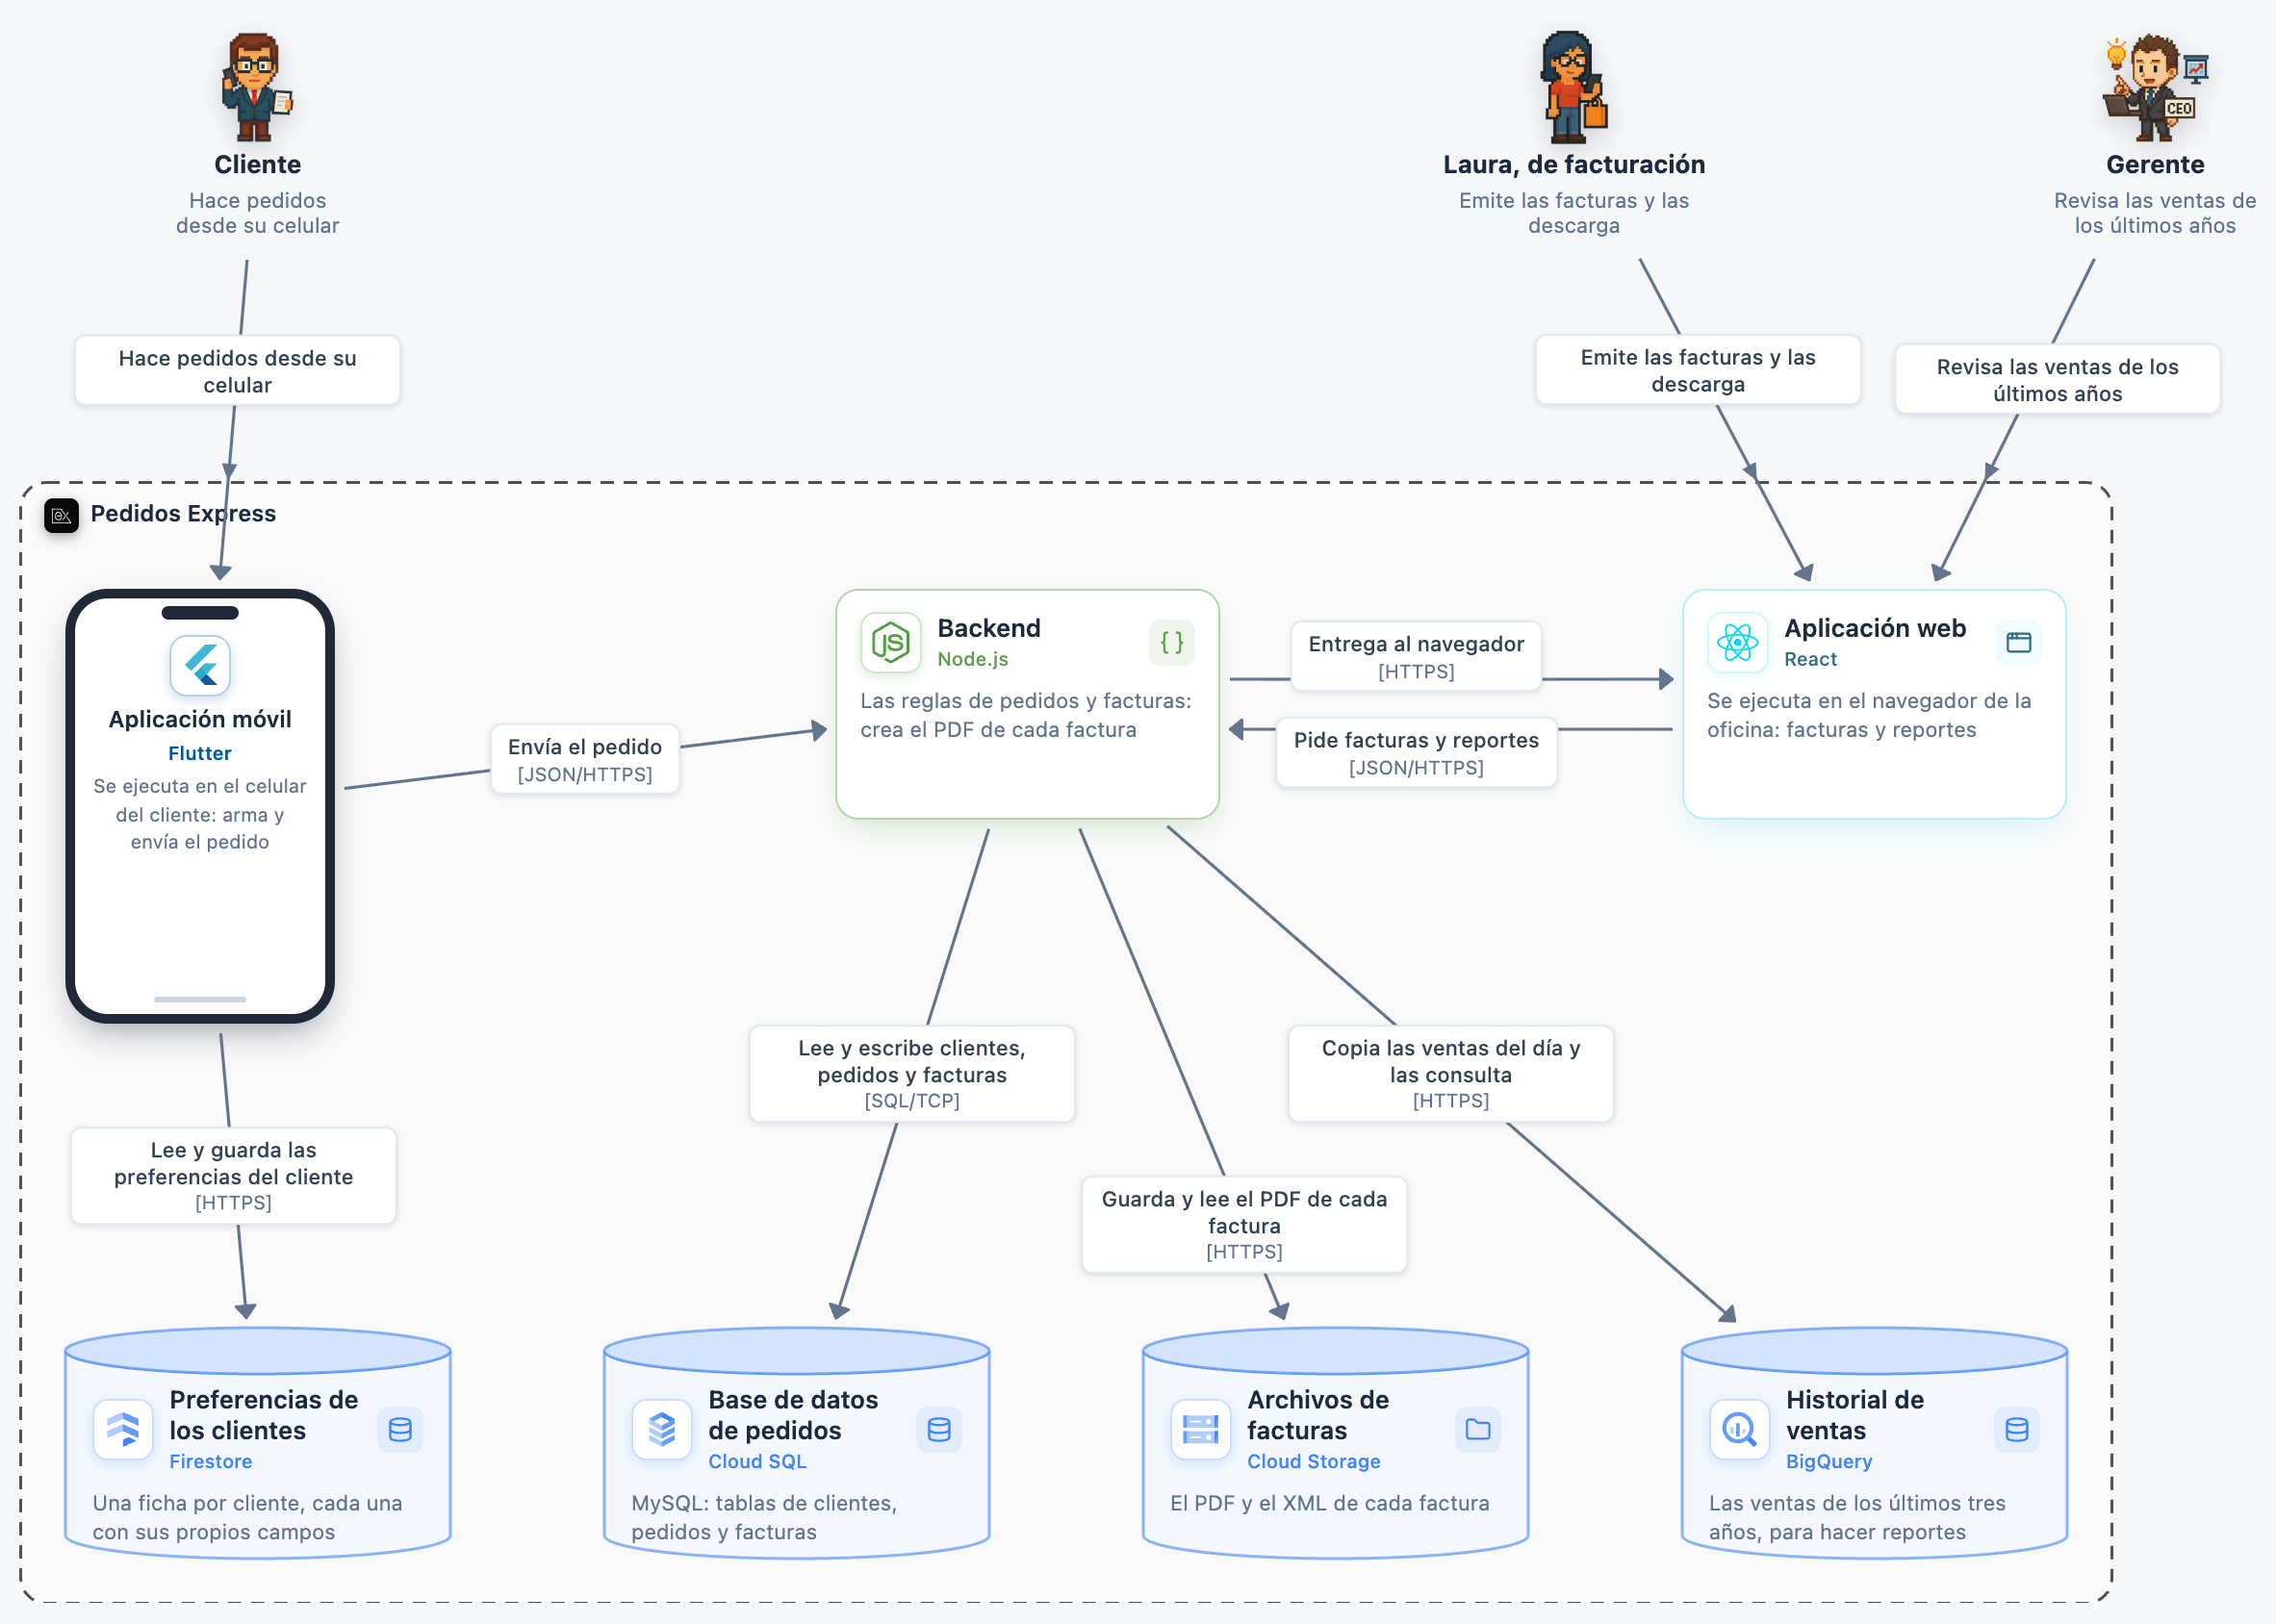
\includegraphics[width=\linewidth]{s23-pedidos-express-datos.png}
\column{.27\textwidth}
\small
\textbf{Cloud SQL}\\clientes, pedidos y facturas\par\medskip
\textbf{Cloud Storage}\\el PDF de cada factura\par\medskip
\textbf{Firestore}\\preferencias de cada cliente\par\medskip
\textbf{BigQuery}\\ventas de tres años\par\vspace{3mm}
\begin{exampleblock}{Empieza simple}
\small Para una webapp, el primer paso casi siempre es \textbf{Cloud SQL}.
\end{exampleblock}
\end{columns}
\end{frame}

% 12
\begin{frame}{Cloud SQL: tres motores para elegir}
\begin{center}
\begin{tikzpicture}[font=\small,
 motor/.style={draw=utpRojo,thick,rounded corners=4pt,fill=utpRojo!10,minimum height=2.1cm,align=center,text width=3.7cm,execute at begin node={\hyphenpenalty=10000}}]
  \node[motor,fill=utpRojo!25] at (0,0) {\textbf{\large MySQL}\\[3pt]\footnotesize Libre y muy popular en webapps.\\El lab usa MySQL 8.0};
  \node[motor] at (4.5,0) {\textbf{\large PostgreSQL}\\[3pt]\footnotesize Libre y muy completo:\\más tipos de datos y reglas};
  \node[motor] at (9.0,0) {\textbf{\large SQL Server}\\[3pt]\footnotesize De Microsoft, con licencia:\\común en empresas};
\end{tikzpicture}
\end{center}
\begin{block}{Lo eliges al crear la instancia}
\small En el lab hiciste clic en \textbf{Elegir MySQL}. Sea cual sea el motor, Google lo instala, lo actualiza y hace sus copias de seguridad.
\end{block}
\begin{alertblock}{Los tres son relacionales}
\small Guardan tablas y se consultan con SQL. Cambia el motor, no la idea.
\end{alertblock}
\end{frame}

% 13
\begin{frame}{¿SQLite, MySQL, PostgreSQL o SQL Server?}
\renewcommand{\arraystretch}{1.3}
\centering\small
\begin{tabular}{@{}p{2.1cm}>{\raggedright\arraybackslash}p{3.6cm}>{\raggedright\arraybackslash}p{4.0cm}>{\raggedright\arraybackslash}p{3.0cm}@{}}
\toprule
\textbf{Motor} & \textbf{Cómo funciona} & \textbf{Úsalo cuando\ldots} & \textbf{Ejemplo}\\
\midrule
\textbf{SQLite} & Un archivo dentro de la app, sin servidor & La app es pequeña o trabaja sola: prototipos, apps móviles & Los contactos de tu celular\\
\textbf{MySQL} & Un servidor, libre & Haces una webapp o tienda y quieres lo más conocido & WordPress, como en el lab\\
\textbf{PostgreSQL} & Un servidor, libre & Necesitas datos más ricos: mapas, JSON, reglas estrictas & Una app de reparto con mapas\\
\textbf{SQL Server} & Un servidor de Microsoft, con licencia & La empresa ya trabaja con Windows y .NET & El sistema interno de un banco\\
\bottomrule
\end{tabular}
\par\vspace{3mm}
\begin{alertblock}{En Google Cloud}
\small Los cuatro hablan SQL. Cloud SQL ofrece MySQL, PostgreSQL y SQL Server. SQLite no: viaja dentro de la aplicación, no es un servidor.
\end{alertblock}
\end{frame}

% 14
\separador{Parte 2: Cloud SQL en el lab}{Una base de datos y dos WordPress conectados a ella}

% 12
\begin{frame}{El lab en cuatro pasos}
\renewcommand{\arraystretch}{1.4}
\centering\small
\begin{tabular}{@{}p{0.5cm}>{\raggedright\arraybackslash}p{3.6cm}>{\raggedright\arraybackslash}p{8.4cm}@{}}
\toprule
 & \textbf{Tarea} & \textbf{En palabras simples}\\
\midrule
1 & Crear la instancia & Pides a Google un servidor MySQL llamado \texttt{wordpress-db}. Google lo instala y lo cuida.\\
2 & Configurar el proxy & En la VM \texttt{wordpress-proxy} pones un programa que abre un túnel seguro hacia la base. Creas la base \texttt{wordpress}.\\
3 & Conectar WordPress & Instalas WordPress y le dices que la base está en \texttt{127.0.0.1}: ahí lo espera el proxy.\\
4 & Usar la IP privada & Otra VM, en la misma red, se conecta directo a la base, sin proxy.\\
\bottomrule
\end{tabular}
\par\vspace{3mm}
\begin{alertblock}{Instancia y base de datos}
\small \texttt{wordpress-db} es el servidor, como un edificio. \texttt{wordpress} es una base dentro de él, como una oficina.
\end{alertblock}
\end{frame}

% 13
\begin{frame}{El lab en un diagrama}
\begin{columns}[c,onlytextwidth]
\column{.68\textwidth}
\centering
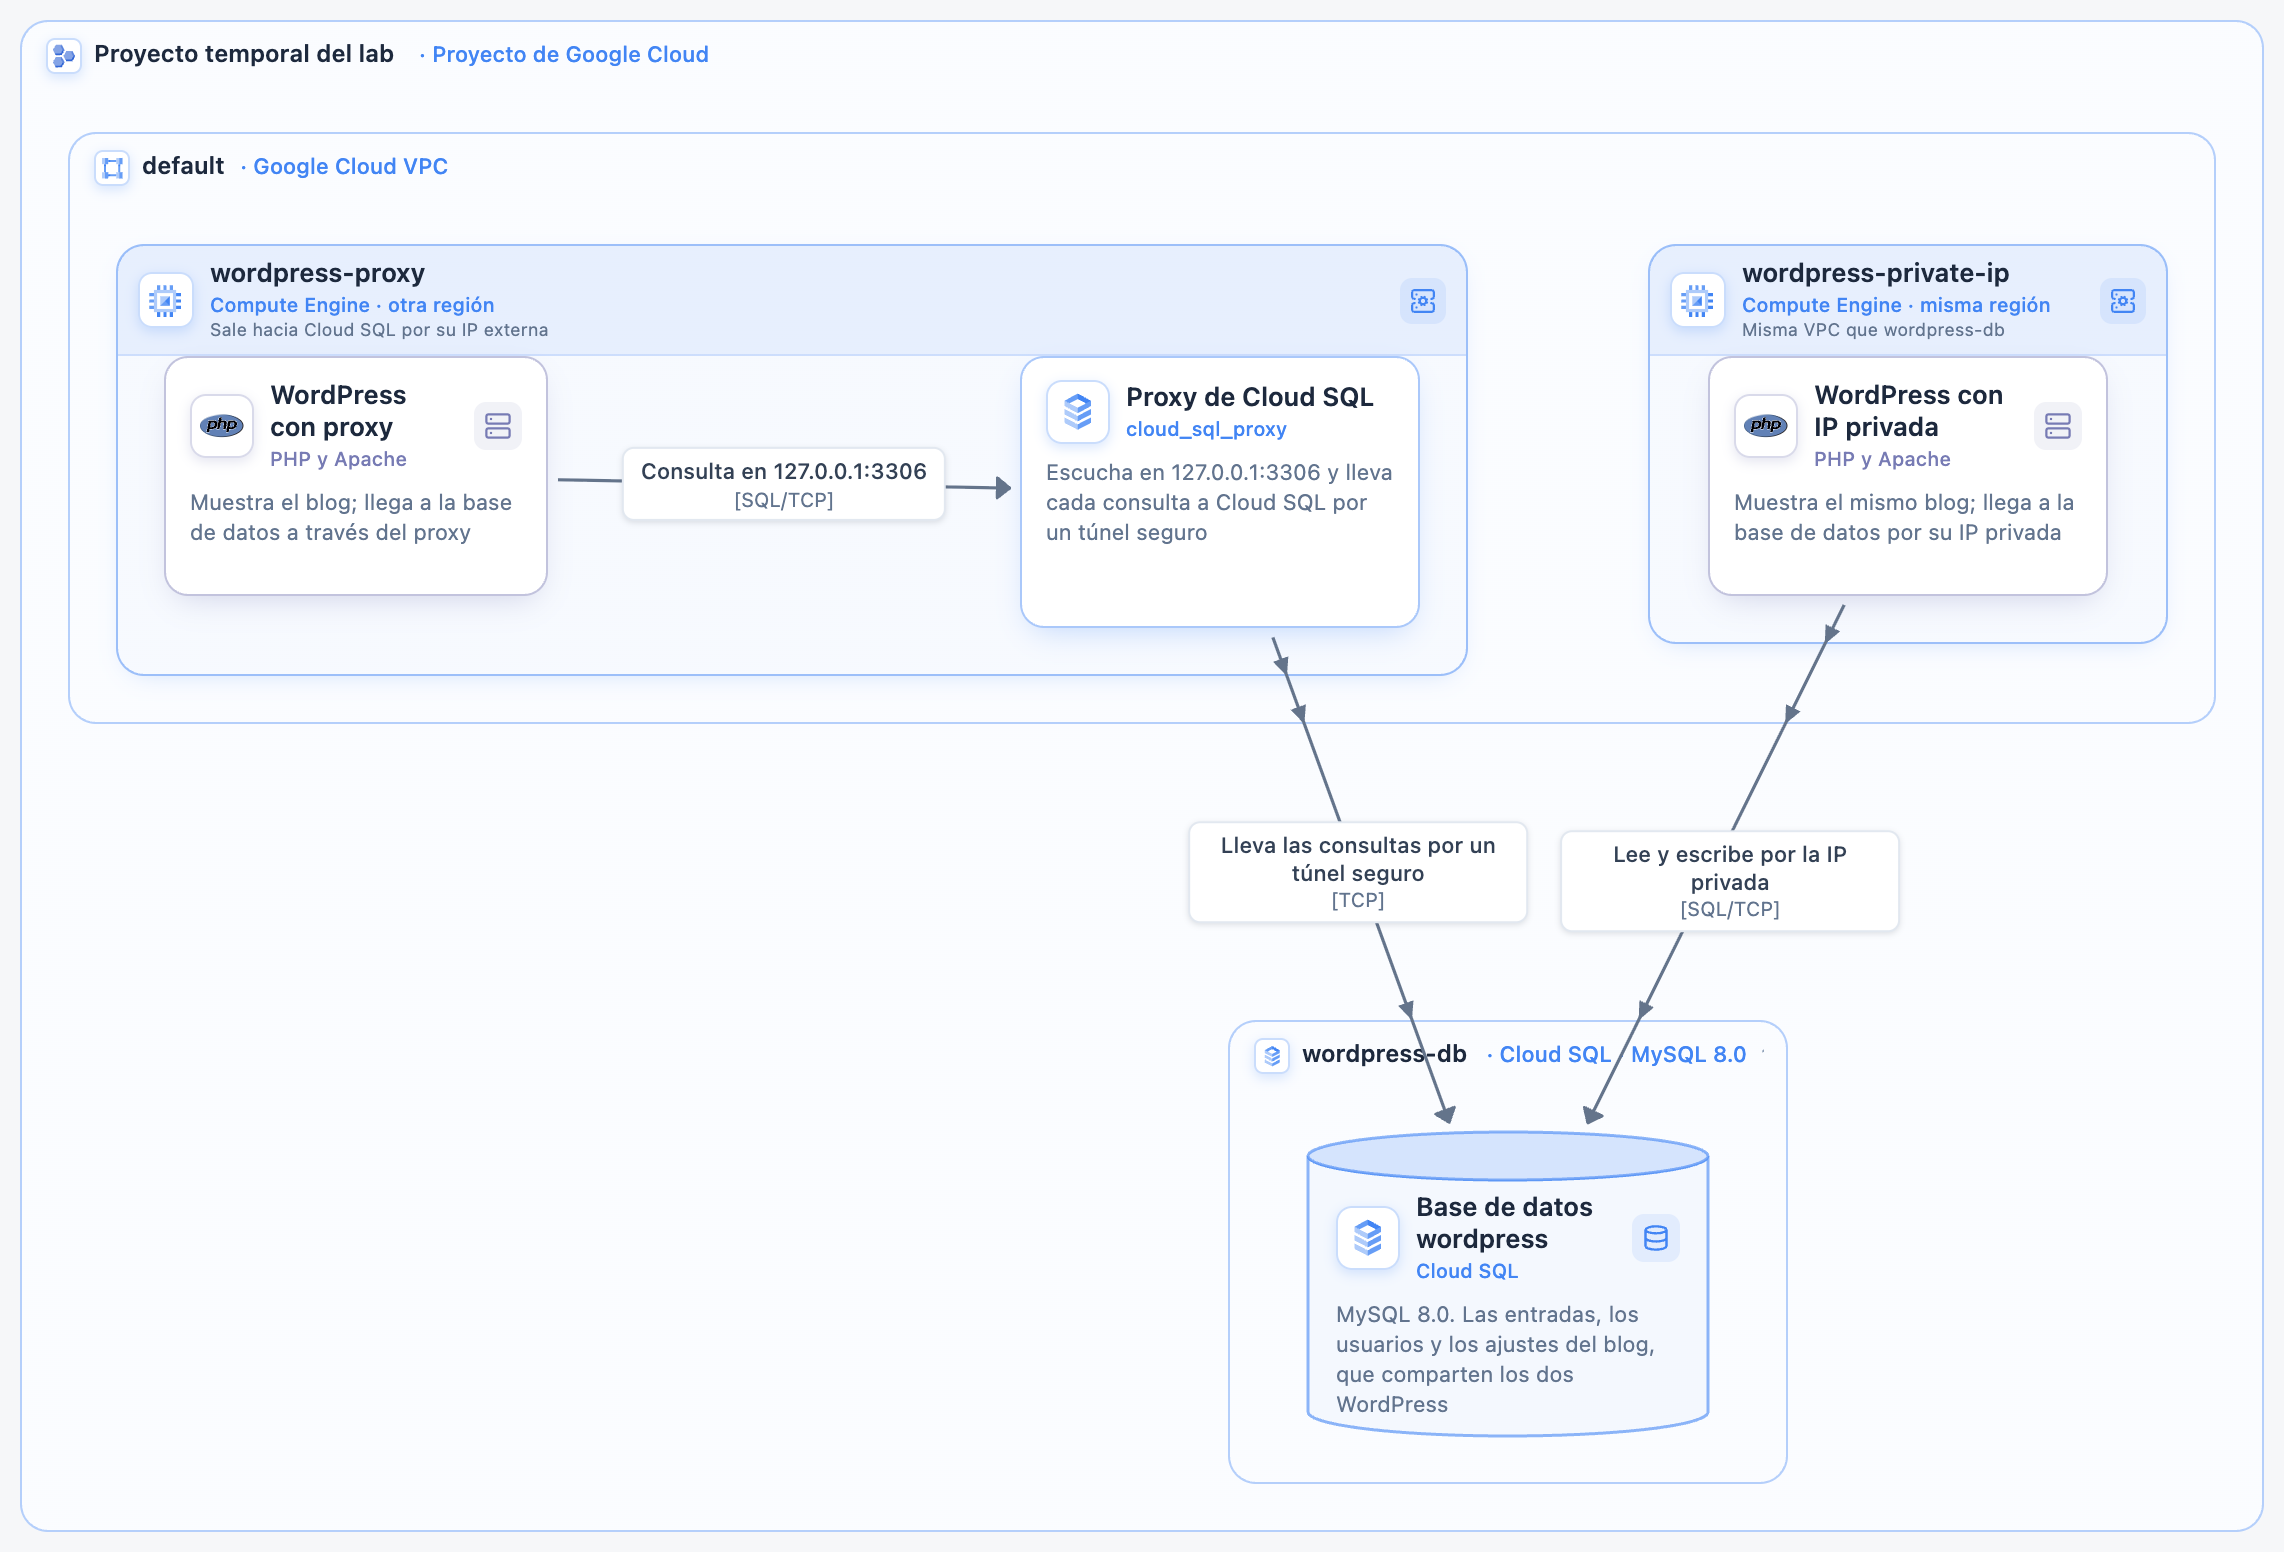
\includegraphics[width=\linewidth]{s23-lab-cloud-sql.png}
\column{.29\textwidth}
\begin{block}{VM en otra región}
\small Llega a la base con el \textbf{proxy}.
\end{block}
\begin{block}{VM en la misma región y red}
\small Llega directo por la \textbf{IP privada}: más rápido y no sale a Internet.
\end{block}
\begin{exampleblock}{\textit{Already Installed!}}
\small El segundo WordPress encontró el blog que creó el primero: los dos usan la \textbf{misma} base.
\end{exampleblock}
\end{columns}
\end{frame}

% 14
\begin{frame}[c]{Práctica}
\begin{block}{Realiza el laboratorio}
\large \textit{Implementa Cloud SQL}\par\vspace{1mm}
\small\texttt{skills.google/paths/11/course\_templates/49/labs/592108}
\end{block}
\begin{exampleblock}{Al terminar}
\small Ves el mismo blog de WordPress desde las dos VMs.
\end{exampleblock}
\end{frame}

% 15
\begin{frame}{Cierre: preguntas para comprobar}
\begin{block}{Responde con tus palabras}
\small
1. ¿Qué diferencia hay entre una base relacional y una no relacional?\\\medskip
2. En Pedidos Express, ¿dónde va la fila de la factura y dónde va su PDF?\\\medskip
3. ¿Qué servicio usarías para analizar tres años de ventas?\\\medskip
4. En el lab, ¿por qué el segundo WordPress mostró \textit{Already Installed!}?
\end{block}
\begin{alertblock}{Idea final}
\small Elige la base según la forma de tus datos y su uso. Para una webapp típica, Cloud SQL: una base relacional que Google administra.
\end{alertblock}
\end{frame}

% 16
\begin{frame}{Referencias}
\scriptsize
\begin{itemize}\setlength\itemsep{4pt}
  \item Laboratorio: \textit{Implementa Cloud SQL}, curso \textit{Essential Google Cloud Infrastructure: Core Services}: \texttt{skills.google/paths/11/course\_templates/49/labs/592108}.
  \item Diagramas de la sesión, en SystemModeler: \texttt{ejemplos/pedidos\_express} y \texttt{ejemplos/wordpress\_con\_cloud\_sql}.
  \item Material previo del curso: Sesión 21, arquitectura inicial de una webapp; Sesión 22, IAM y cuentas de servicio.
  \item Google Cloud: Cloud SQL, Spanner, Firestore, Bigtable, BigQuery y Cloud Storage.
  \item Las respuestas de las preguntas están en \texttt{../respuestas.md}.
\end{itemize}
\end{frame}

\end{document}
